\begin{figure}[]
\centering     
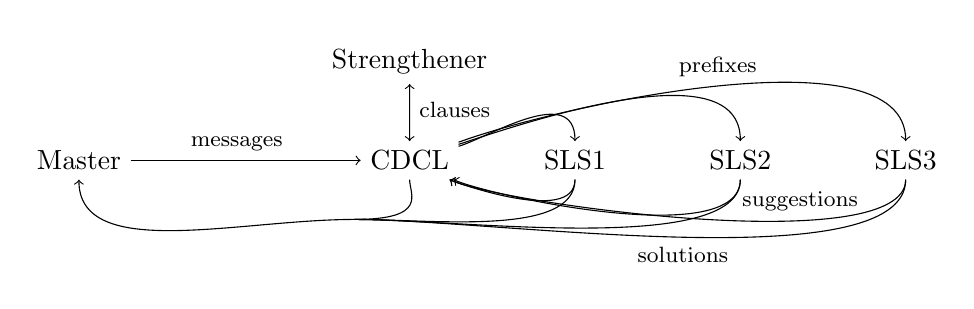
\begin{tikzpicture}[xscale=0.7,yscale=-0.5]

\node (master)	at (-3.0,4.0)	[align=center] {Master};

%\node (worker_group_label1)	at (-1.1,1.3)	[above,gray] {Worker group 1};
%\draw [gray]  (1.0,0.5) -- (14.0,0.5) -- (14.0,7.0) -- (1.0,7.0) -- cycle ;
\node (strengthener1)	at (3.0,1.5)	[align=center] {Strengthener};
\node (tinisat1)		at (3.0,4.0)	[align=center] {CDCL};
\node (gnovelty11)	at (6.0,4.0)	[align=center] {SLS1};
\node (gnovelty12)	at (9.0,4.0)	[align=center] {SLS2};
\node (gnovelty13)	at (12.0,4.0)	[align=center] {SLS3};
\draw [-,out=0,in=180,looseness=0.15] (master.east) to (-0.5,4.0);
\draw [->,out=0,in=180,looseness=0.75] (-0.5,4.0) to node[above,pos=0.15]{\footnotesize messages} (tinisat1);
\draw [-,out=90,in=0,looseness=1.55] (tinisat1) to (2.0,5.5);
\draw [->,out=180,in=90,looseness=1.05] (2.0,5.5) to  (master.south);
\draw [-,out=90,in=0,looseness=0.90] (gnovelty11.south) to (2.0,5.5);
\draw [-,out=90,in=0,looseness=0.70] (gnovelty12.south) to (2.0,5.5);
\draw [-,out=90,in=0,looseness=0.65] (gnovelty13.south) to node[below,pos=0.5]{\footnotesize solutions} (2.0,5.5);
\draw [->,out=315,in=270,looseness=1.35] (tinisat1) to (gnovelty11.north);
\draw [->,out=320,in=270,looseness=1.05] (tinisat1) to (gnovelty12.north);
\draw [->,out=320,in=270,looseness=0.85] (tinisat1) to node[above,pos=0.5]{\footnotesize prefixes} (gnovelty13.north);
\draw [<->,out=270,in=90,looseness=1.55] (tinisat1) to node[right,pos=0.8]{\footnotesize clauses} (strengthener1.south);


\draw [->,out=90,in=60,looseness=1.02] (gnovelty11.south) to (tinisat1);
\draw [->,out=90,in=50,looseness=0.80] (gnovelty12.south) to (tinisat1);
\draw [->,out=90,in=50,looseness=0.60] (gnovelty13.south) to node[above,pos=0.33]{\footnotesize suggestions} (tinisat1);

\end{tikzpicture}
\caption[Messages between components in \dagster\ ]{Relationship and messages between the master and worker groups within \dagster}\label{fig:dagster_organisation}
\end{figure}
